\section{Background and Motivation}
\label{sec:motivation}

\subsection{Task views and reusable state}

A coding-agent workspace contains source files, dependencies, generated
artifacts, and temporary files. In the deployment considered here, multiple
attempts can start from a common repository revision and dependency set.
For example, two attempts may initially read the same \code{src/parser.py}.
If one edits or deletes that file, the other must continue to see its own
version. The shared starting state must therefore have a stable identity,
and each attempt's changes must remain private. This is a requirement on
the visible file tree, independent of where its metadata and bytes reside.

Reuse is conditional on the deployment. A stable dependency tree may serve
many attempts, whereas generated outputs may be replaced on every run.
A baseline can cover a selected subtree; it need not include the entire
working directory. The value of sharing depends on overlap between tasks,
the amount of private modification, and how long the baseline remains
useful. These properties determine whether sharing is appropriate; they
are distinct from the access behavior of an individual task.

\subsection{From file operations to storage work}

To read \code{src/parser.py}, a tool first needs the path resolved and the
file's data located. An object-backed file system keeps names, attributes,
and file-to-object mappings in its metadata path, and retrieves payloads
from caches or object storage. Metadata services can batch requests and
cache records~\cite{tablefs2013,indexfs2014}; immutable distributions can
also organize records for demand fetching~\cite{cvmfs2011,nydus_rafs}.
Resolving a shared file therefore does not imply either a network request
per metadata operation or a particular metadata representation.

The requested file range also differs from the storage work it induces.
Kernel caching and readahead affect which requests reach FUSE. The client
then maps those requests to stored objects and may fetch a range or an
entire object. Backend encoding and integrity checks can require access
to still different units~\cite{azureec2012,okapi2025}. Writes similarly
pass through buffering and object formation before publication. Thus a
small file request does not by itself determine transferred bytes,
verification work, or uploaded object size. The following observations
characterize one point in this path: requests received by FUSE handlers.

\subsection{Observed requests in real agent runs}
\label{sec:agent-observations}

\paragraph{Capture and scope.}
We reanalyzed eight SWE-bench Verified task runs~\cite{swebench2024}: five
Core and three Exploratory. All used DSH 0.1.5-rc.1 and the CCSwitch-configured
model \code{deepseek-v4-flash}. Exploratory runs used a broader
investigation/testing prompt and a 30-minute budget; all finished earlier.
Each base-commit checkout was mounted through \code{libfuse-fs}
\code{PassthroughFs} on Ubuntu 24.04 under WSL; \code{rfuse3}
\code{LoggingFileSystem} recorded actual FUSE handler requests.
Streaming reanalysis covered all 1,138,884 events: 217,129 Core and 921,755
Exploratory. Counts retain every status, 64 setup/canary requests before
agent startup, and teardown, including 24 requests after recorded run finish.
Group statistics weight requests equally, not tasks. Per-task counts and
source-validation details are in the companion workload record.

\begin{figure*}[!t]
\centering
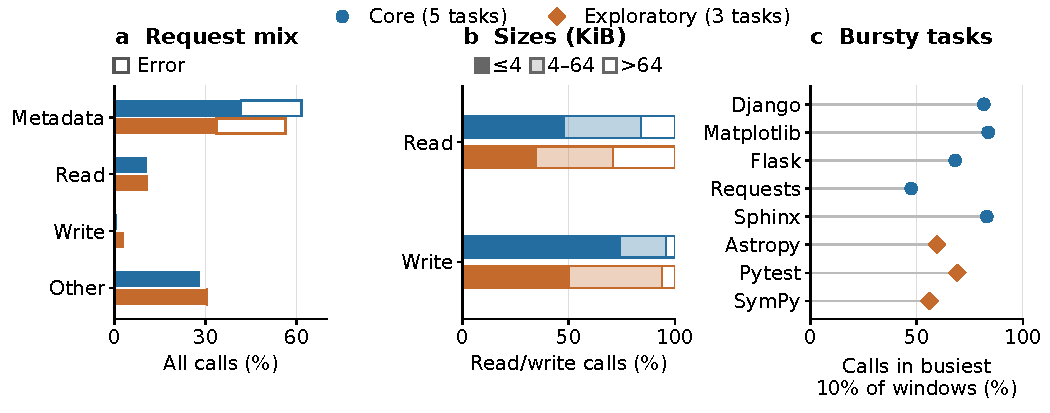
\includegraphics[width=\textwidth]{figures/agent-fuse/fuse-combined-compact.pdf}
\caption{Request structure across eight single-run FUSE captures.
Core bars precede Exploratory bars in each pair.
(a) Shares of all calls; white segments are errors within each total.
Metadata comprises \code{lookup}, \code{getattr}, \code{getxattr},
\code{readdirplus}, \code{opendir}, and \code{releasedir}; Other contains
every remaining method, including file open/flush/release.
(b) Each bar includes all reads or writes in its group. Dark, light, and white
segments denote $\leq4$, $(4,64]$, and $>64$ KiB, respectively
($1\,\mathrm{KiB}=1024$ bytes). Read counts are 22,142/98,292 and write
counts 1,112/23,600 (Core/Exploratory), all \code{ok}. Lengths are requested
FUSE bytes, not object sizes.
(c) Fraction of each task's calls in its busiest 10\% of one-second windows,
rounding the window count up; zero-call and final partial windows are retained.
All panels retain setup/teardown and every recorded status.}
\label{fig:agent-fuse-combined}
\end{figure*}

\paragraph{Metadata traffic and read dominance.}
The six metadata methods accounted for 61.5\% of Core and 56.4\%
of Exploratory calls (Figure~\ref{fig:agent-fuse-combined}a).
Restricting the denominator and numerator to \code{ok} events reduces these
shares to 52.0\% and 44.2\%: failed probes materially change the request mix.
Across tasks, the all-status share ranged from 39.6\% in SymPy to 65.4\% in
Django, so the group majority does not describe every task.
Read calls outnumbered writes by 19.9:1 in Core and 4.16:1 in Exploratory;
per-task ratios ranged from 3.12:1 (Pytest) to 42.7:1 (Matplotlib).
These observations motivate evaluating both positive and negative metadata
paths alongside data I/O.

\paragraph{A mixture of request sizes.}
Reads ranged from 4 to 128 KiB, with Core and Exploratory medians of 8 and
16 KiB. Writes ranged from one byte
to 128 KiB, with medians of 4,084 and 4,117 bytes, respectively.
Requests of at most 4 KiB accounted for 47.7\% and 34.5\% of reads, and
74.3\% and 49.9\% of writes. The interval $(4,64]$ KiB contained a further
36.2\% and 36.4\% of reads and 21.3\% and 44.0\% of writes
(Figure~\ref{fig:agent-fuse-combined}b).
This mixture motivates measuring how client fetching and uploads transform
requests before testing backend layouts. FUSE observations occur below kernel
caching and readahead; they do not identify application syscall sizes, unique
bytes, finalized object lengths, or an optimal block size.

\paragraph{Task and temporal heterogeneity.}
Tasks generated 8,542--634,726 calls. Astropy contributed 68.9\% of
Exploratory calls, versus 6.0\% for Pytest. Capture spans, from first to last
request start, were 42.7--71.3 seconds for Core and 119.9--556.1 seconds for
Exploratory. The busiest 10\% of one-second windows, rounded up per task,
contained 47.4--83.7\% of its calls (Figure~\ref{fig:agent-fuse-combined}c).
The companion record retains the full method breakdowns, size ECDFs,
and per-task cumulative time curves. Replay
should retain these per-task mixes and bursts. Each task was observed once;
different repositories, prompts, and budgets prevent a causal interpretation
of the group contrast. Without tool-phase labels, bursts cannot be assigned
to searching, editing, or testing.

\paragraph{Status semantics and evidence limits.}
The capture contained 872,519 \code{ok}, 253,669 \code{error}, and 12,696
\code{incomplete} events. Errors occurred in \code{lookup} (233,452),
\code{getxattr} (20,203), and \code{rmdir} (14). Collection notes associate
many with failed path probes or unsupported attributes; absent errno values
prevent event-level cause attribution. The parser labels a request
\code{incomplete} when no recognized completion is paired with it: here,
12,688 \code{forget} and eight \code{destroy} records. Neither label counts
failed agent tasks. All eight agent and daemon exit codes were zero, which
does not establish SWE-bench grading success.

Handler latency measures WSL passthrough intervals and excludes model response
time. Elapsed capture time instead includes inter-request gaps, which may
contain model waiting; summing overlapping handler intervals cannot recover
task wall time. These observations do not measure RustFS, Redis, network
object storage, or cloud-disk latency. They motivate metadata and mixed-I/O
experiments for this single-agent/model panel, but do not establish cross-task
sharing, sparse mutation, or performance gains from \sysname, RustFS, or
the automatic hint policy. Those remain questions for
Section~\ref{sec:evaluation}.


\subsection{Implications for storage design}

The observed mix makes metadata resolution a substantial part of the
request path, including unsuccessful probes. It also requires serving
both short and longer data requests, with demand that changes across
tasks and within a run. These observations motivate treating metadata
access and data access as separate design concerns. They do not select
one metadata layout or one object size: grouping can amortize requests
when nearby records or bytes are reused, but can fetch unnecessary data
when accesses are scattered. Whether access savings repay construction
and retention costs depends on how often a version is reused.

The shared-state scenario adds a semantic constraint to these access
choices. A task's private changes must not alter the baseline seen by
other tasks, whatever representation serves that baseline. A reader
that needs only published state should also be able to use its metadata
representation without acquiring a writable workspace. Together, these
requirements motivate separating view composition, immutable metadata
access, and object granularity. Section~\ref{sec:overview} defines the
interfaces through which \sysname{} makes these choices independently
and composes them when a deployment needs more than one.
